\documentclass[10pt]{beamer}

\usetheme[progressbar=foot]{metropolis}

\usepackage{appendixnumberbeamer}
\usepackage{booktabs}
\usepackage[scale=2]{ccicons}
\usepackage{tikz-cd} 
\usepackage{hyperref}
\usepackage{mathtools}
\usepackage{quiver}
\usepackage{stackengine,scalerel}
\newcommand\eye{\ensurestackMath{\stackinset{c}{}{c}{-.33pt}%
		{\bullet}{\bigcirc}}}
\usepackage{graphicx} % Allows including images
\usepackage{bussproofs}
\usepackage{tikz}
\usetikzlibrary{cd}
\usepackage{adjustbox}
\usetikzlibrary{petri,positioning}
\usepackage{booktabs} % Allows the use of \toprule, \midrule and \bottomrule in tables

\usepackage{pgfplots}
\usepgfplotslibrary{dateplot}

\usepackage{xspace}
\newcommand{\themename}{\textbf{\textsc{metropolis}}\xspace}

\title{Timed Alignments}
%\subtitle{A modern beamer theme}
% \date{\today}
\date{}
\author[author] {Thomas Chatain and Neha Rino}
\institute{LMF, ENS Paris-Saclay}
% \titlegraphic{\hfill\includegraphics[height=1.5cm]{logo.pdf}}

\begin{document}

\maketitle

\section[Introduction]{Introduction}

%\begin{frame}[fragile]{Day One}

%	 \includegraphics[width=0.2\textwidth]{employee.png}
%	 \hspace{1.5em}
%%	 	\includegraphics[width= 0.5\textwidth]{airline.jpg}
%\end{frame}

\begin{frame}[fragile]{An example}

\centerline{
	\begin{tabular}{|c| c| c| c|}
		\hline
		Emp ID & Action & Customer ID & timestamp \\ 
		\hline
		1 & reg & 70 & 13:31\\
		2 & reg & 71 & 13:32\\
		1 &et & 70 & 13:32\\
		1& ct & 70 & 13:33\\
		2& reg & 72 & 13:34\\
		2& ec & 71 & 13:34\\
		\hline
	\end{tabular}
}
\vfill 
Register request : reg, Examine thoroughly : et, Examine casually : ec, Check ticket : ct, Decide : dec, Pay : pay, and Reject : rej. 

\end{frame}
\begin{frame}
	Group by customer ID, throw away other details : 
	\vfill 
	
	\centerline{
		\begin{tabular}{|c| c| }
			\hline
			Customer ID & Action \\ 
			\hline
			70 &  reg \\
			70 & et \\
			70 & ct \\
			70 & dec \\
			70 & pay \\
			\hline
			71 & reg \\
			71 & ec \\
			71 & ct \\
			71 & dec\\
			71 & rej \\
			\hline
			72 & reg\\
			72&ct\\
			\hline
		\end{tabular}
	}
	
\end{frame}


\begin{frame}[fragile]{Process Mining}

Perhaps, we deduce the following process model : \vfill 
\adjustbox{scale=0.7}{
	\begin{tikzcd}
		&& {\Huge{\bigcirc}} & {\fbox{et}} & {\Huge{\bigcirc}} &&& {\fbox{pay}} \\
		{\Huge{\bigcirc}} & {\fbox{reg}} && {\fbox{ec}} && {\fbox{dec}} & {\Huge{\bigcirc}} && {\Huge{\bigcirc}} \\
		&& {\Huge{\bigcirc}} & {\fbox{ct}} & {\Huge{\bigcirc}} &&& {\fbox{rej}}\\
		\arrow[from=2-1, to=2-2]
		\arrow[curve={height=-12pt}, from=2-2, to=1-3]
		\arrow[curve={height=12pt}, from=2-2, to=3-3]
		\arrow[from=1-3, to=1-4]
		\arrow[from=1-4, to=1-5]
		\arrow[from=3-3, to=3-4]
		\arrow[from=3-4, to=3-5]
		\arrow[curve={height=12pt}, from=3-5, to=2-6]
		\arrow[curve={height=-12pt}, from=1-5, to=2-6]
		\arrow[from=2-6, to=2-7]
		\arrow[curve={height=-12pt}, from=2-7, to=1-8]
		\arrow[curve={height=12pt}, from=2-7, to=3-8]
		\arrow[curve={height=12pt}, from=1-3, to=2-4]
		\arrow[curve={height=12pt}, from=2-4, to=1-5]
		\arrow[curve={height=-12pt}, from=1-8, to=2-9]
		\arrow[curve={height=12pt}, from=3-8, to=2-9]
	\end{tikzcd}
}


\end{frame}

\begin{frame}{Timestamps}
	But sometimes, we want to retain the timing information :   
	\vfill 
	
	\centerline{
	\begin{tabular}{|c| c| c|}
		\hline
		Customer ID & Action & timestamp \\ 
		\hline
		70 &  reg & 13:31\\
		70 & et & 13:32\\
		70 & ct & 13:33\\
		70 & dec & 13:37\\
		70 & pay & 13:38\\
		\hline
		71 & reg & 13:32\\
		71 & ec & 13:34\\
		71 & ct & 13:34\\
		71 & dec & 13:36\\
		71 & rej & 13:36\\
		\hline
		72 & reg & 13:34\\
		72 & ct & 13:36\\
		\hline
	\end{tabular}
}

	
\end{frame}
\begin{frame}[fragile]{Time Constraints : Time Petri Nets}
Now, maybe we could have a process model like : 
\vfill 
\adjustbox{scale=0.7}{
\begin{tikzcd}
	& {} & \Huge\bigcirc & {\fbox{ec}} & \Huge\bigcirc & {} && {\fbox{pay}} \\
	\Huge\bigcirc & {\fbox{reg}} && {\fbox{et}} && {\fbox{dec}} & \Huge\bigcirc & {} & \Huge\bigcirc \\
	&& \Huge\bigcirc & {\fbox{ct}} & \Huge\bigcirc &&& {\fbox{rej}}
	\arrow["{[0, \infty]}"{description, pos=0.2}, shift left=3, draw=white, from=2-2, to=1-2]
	\arrow[""{name=0, anchor=center, inner sep=0}, "{[2,2]}"{description, pos=0.1}, draw=white, from=2-4, to=1-4]
	\arrow["{[2,2]}"{description, pos=0.1}, draw=white, from=3-4, to=2-4]
	\arrow["{[2,4]}"{description, pos=0.1}, shift right=4, draw=white, from=2-6, to=1-6]
	\arrow["{[0,1]}"{description, pos=0.1}, draw=white, from=1-8, to=2-8]
	\arrow["{[0,0]}"{description, pos=0.1}, draw=white, from=3-8, to=2-8]
	\arrow[from=2-1, to=2-2]
	\arrow[curve={height=-12pt}, from=2-2, to=1-3]
	\arrow[curve={height=12pt}, from=2-2, to=3-3]
	\arrow[from=1-3, to=1-4]
	\arrow[from=1-4, to=1-5]
	\arrow[curve={height=12pt}, from=1-3, to=2-4]
	\arrow[curve={height=12pt}, from=2-4, to=1-5]
	\arrow[from=3-3, to=3-4]
	\arrow[from=3-4, to=3-5]
	\arrow[curve={height=-12pt}, from=1-5, to=2-6]
	\arrow[curve={height=12pt}, from=3-5, to=2-6]
	\arrow[from=2-6, to=2-7]
	\arrow[curve={height=-12pt}, from=2-7, to=1-8]
	\arrow[curve={height=12pt}, from=2-7, to=3-8]
	\arrow[curve={height=12pt}, from=3-8, to=2-9]
	\arrow[curve={height=-12pt}, from=1-8, to=2-9]
	\arrow["{[0,2]}"{description, pos=0.2}, draw=white, from=1-4, to=0]
\end{tikzcd}
}
\end{frame}

%\begin{frame}[fragile]{Processes, Event Logs and Models}
	
%\huge{$$Model \xLeftrightarrow[Checking]{Conformance}  Event Log$$}
	
%\end{frame}


\subsection{Conformance Checking}

\begin{frame}{Conformance Checking}
    \begin{itemize}
        \item Relating observed and modelled behaviour [CarmonaDSW18]
        \vfill 
        \item Evaluate a process model, or correct an event log using precision, fitness, simplicity, generalisation, etc
        \vfill 
        \item Fitness : Does model represent the process well? 

    \end{itemize}
        \vfill 
$$Log \subseteq \mathcal{L}(N)$$
\end{frame}

\begin{frame}[fragile]{Alignments}
	
	\adjustbox{scale=0.7}{
		\begin{tikzcd}
			&& {\Huge{\bigcirc}} & {\fbox{et}} & {\Huge{\bigcirc}} &&& {\fbox{pay}} \\
			{\Huge{\bigcirc}} & {\fbox{reg}} && {\fbox{ec}} && {\fbox{dec}} & {\Huge{\bigcirc}} && {\Huge{\bigcirc}} \\
			&& {\Huge{\bigcirc}} & {\fbox{ct}} & {\Huge{\bigcirc}} &&& {\fbox{rej}}\\
			\arrow[from=2-1, to=2-2]
			\arrow[curve={height=-12pt}, from=2-2, to=1-3]
			\arrow[curve={height=12pt}, from=2-2, to=3-3]
			\arrow[from=1-3, to=1-4]
			\arrow[from=1-4, to=1-5]
			\arrow[from=3-3, to=3-4]
			\arrow[from=3-4, to=3-5]
			\arrow[curve={height=12pt}, from=3-5, to=2-6]
			\arrow[curve={height=-12pt}, from=1-5, to=2-6]
			\arrow[from=2-6, to=2-7]
			\arrow[curve={height=-12pt}, from=2-7, to=1-8]
			\arrow[curve={height=12pt}, from=2-7, to=3-8]
			\arrow[curve={height=12pt}, from=1-3, to=2-4]
			\arrow[curve={height=12pt}, from=2-4, to=1-5]
			\arrow[curve={height=-12pt}, from=1-8, to=2-9]
			\arrow[curve={height=12pt}, from=3-8, to=2-9]
		\end{tikzcd}
	}

	\begin{itemize}
		\item Suppose we observe the trace \alert{$$reg \cdot et \cdot et \cdot ct \cdot dec \cdot pay$$} 
		\vfill 
		\item Aligning word : \alert{$$reg \cdot et \cdot ct \cdot dec \cdot pay$$}
	\end{itemize}

\end{frame}


\begin{frame}[fragile]{Timed Alignments}
\adjustbox{scale=0.7}{
\begin{tikzcd}
	& {} & \Huge\bigcirc & {\fbox{ec}} & \Huge\bigcirc & {} && {\fbox{pay}} \\
	\Huge\bigcirc & {\fbox{reg}} && {\fbox{et}} && {\fbox{dec}} & \Huge\bigcirc & {} & \Huge\bigcirc \\
	&& \Huge\bigcirc & {\fbox{ct}} & \Huge\bigcirc &&& {\fbox{rej}}
	\arrow["{[0, 1]}"{description, pos=0.2}, shift left=3, draw=white, from=2-2, to=1-2]
	\arrow[""{name=0, anchor=center, inner sep=0}, "{[2,2]}"{description, pos=0.1}, draw=white, from=2-4, to=1-4]
	\arrow["{[2,2]}"{description, pos=0.1}, draw=white, from=3-4, to=2-4]
	\arrow["{[2,4]}"{description, pos=0.1}, shift right=4, draw=white, from=2-6, to=1-6]
	\arrow["{[0,1]}"{description, pos=0.1}, draw=white, from=1-8, to=2-8]
	\arrow["{[0,0]}"{description, pos=0.1}, draw=white, from=3-8, to=2-8]
	\arrow[from=2-1, to=2-2]
	\arrow[curve={height=-12pt}, from=2-2, to=1-3]
	\arrow[curve={height=12pt}, from=2-2, to=3-3]
	\arrow[from=1-3, to=1-4]
	\arrow[from=1-4, to=1-5]
	\arrow[curve={height=12pt}, from=1-3, to=2-4]
	\arrow[curve={height=12pt}, from=2-4, to=1-5]
	\arrow[from=3-3, to=3-4]
	\arrow[from=3-4, to=3-5]
	\arrow[curve={height=-12pt}, from=1-5, to=2-6]
	\arrow[curve={height=12pt}, from=3-5, to=2-6]
	\arrow[from=2-6, to=2-7]
	\arrow[curve={height=-12pt}, from=2-7, to=1-8]
	\arrow[curve={height=12pt}, from=2-7, to=3-8]
	\arrow[curve={height=12pt}, from=3-8, to=2-9]
	\arrow[curve={height=-12pt}, from=1-8, to=2-9]
	\arrow["{[0,2]}"{description, pos=0.2}, draw=white, from=1-4, to=0]
\end{tikzcd}
	}
	\vfill 

 Say we observe the timed trace \alert{$$(reg, 1) \cdot (ec, 2) \cdot (ec, 2) \cdot (ct, 3) \cdot (dec, 8) \cdot (rej, 8)$$} 
        \vfill 
        
\definecolor{Brickred}{RGB}{200,60,60}       
\setbeamercolor{block title alerted}{%
    use={block title, alerted text},
    fg = Brickred}
    
 \setbeamercolor{block body alerted}{%
    use={block body, alerted text},
    fg = Brickred}   
\metroset{block=fill}
\begin{alertblock}{Our Goal Today}
         A framework for aligning this observation \end{alertblock}
\end{frame}
%------------------------------------------------
\section{Formal Definitions}


\subsection{Alignments}
\begin{frame}{The Alignment Problem}
\metroset{block=fill}
	\begin{block}{The Alignment Problem [Adriansyah14]}
	Input : A Petri net $N$  and an observed trace $\sigma$
	
	\vfill 
	
	Output : A word $\gamma \in \mathcal{L}(N)$ such that $d(\sigma, \gamma) = \min_{x \in \mathcal{L}(N)} d(\sigma, x)$ for some distance function $d$ on words. 
	\end{block}
\vfill 

Usually $d$ is the Levenshtein edit distance or the Hamming distance. 
\end{frame}

\begin{frame}{The General Timed Alignment Problem}

\metroset{block=fill}
	\begin{block}{GTAP}
		Input : A time Petri net $N$ and an observed timed trace $\sigma$. 
		\vfill 
		
		Output : A timed trace $\alert{\gamma_a}
		\in \mathcal{L}(N)$ such that $d_a(\sigma, \gamma) = \min_{x \in \mathcal{L}(N)} d_a(\sigma, x)$ for some distance function $d_a$ on timed words. 
		\
	\end{block}

\end{frame}

\begin{frame}[fragile]{Example}
\adjustbox{scale=0.7}{	
\begin{tikzcd}
	& {} & \Huge\bigcirc & {\fbox{ec}} & \Huge\bigcirc & {} && {\fbox{pay}} \\
	\Huge\bigcirc & {\fbox{reg}} && {\fbox{et}} && {\fbox{dec}} & \Huge\bigcirc & {} & \Huge\bigcirc \\
	&& \Huge\bigcirc & {\fbox{ct}} & \Huge\bigcirc &&& {\fbox{rej}}
	\arrow["{[0, 1]}"{description, pos=0.2}, shift left=3, draw=white, from=2-2, to=1-2]
	\arrow[""{name=0, anchor=center, inner sep=0}, "{[2,2]}"{description, pos=0.1}, draw=white, from=2-4, to=1-4]
	\arrow["{[2,2]}"{description, pos=0.1}, draw=white, from=3-4, to=2-4]
	\arrow["{[2,4]}"{description, pos=0.1}, shift right=4, draw=white, from=2-6, to=1-6]
	\arrow["{[0,1]}"{description, pos=0.1}, draw=white, from=1-8, to=2-8]
	\arrow["{[0,0]}"{description, pos=0.1}, draw=white, from=3-8, to=2-8]
	\arrow[from=2-1, to=2-2]
	\arrow[curve={height=-12pt}, from=2-2, to=1-3]
	\arrow[curve={height=12pt}, from=2-2, to=3-3]
	\arrow[from=1-3, to=1-4]
	\arrow[from=1-4, to=1-5]
	\arrow[curve={height=12pt}, from=1-3, to=2-4]
	\arrow[curve={height=12pt}, from=2-4, to=1-5]
	\arrow[from=3-3, to=3-4]
	\arrow[from=3-4, to=3-5]
	\arrow[curve={height=-12pt}, from=1-5, to=2-6]
	\arrow[curve={height=12pt}, from=3-5, to=2-6]
	\arrow[from=2-6, to=2-7]
	\arrow[curve={height=-12pt}, from=2-7, to=1-8]
	\arrow[curve={height=12pt}, from=2-7, to=3-8]
	\arrow[curve={height=12pt}, from=3-8, to=2-9]
	\arrow[curve={height=-12pt}, from=1-8, to=2-9]
	\arrow["{[0,2]}"{description, pos=0.2}, draw=white, from=1-4, to=0]
\end{tikzcd}
}	
	
\vfill 
 \begin{itemize}
        \item Recall the observation \alert{$$(reg, 1) \cdot (ec, 2) \cdot (ec, 2) \cdot (ct, 3) \cdot (dec, 8) \cdot (rej, 8)$$} 
        \item One guess : \alert{$(reg, 1) \cdot (ec, 2) \cdot (ct, 3) \cdot (dec, 7) \cdot (rej, 7)$} 
        \vfill 
        \item Another : \alert{$(reg, 1) \cdot (ec, 2) \cdot (ct, 3) \cdot (dec, 7) \cdot (pay, 8)$} 
    \end{itemize}
\end{frame}

\begin{frame}{The Purely Timed Alignment Problem}
	\metroset{block = fill}
	\begin{block}{PTAP}
		Input : A time Petri net $N$ and an observed timed trace $(w, \sigma)$ and a valid causal process of the untimed part $w$. 
		\vfill 
		
		Output : A valid timing function $\alert{\gamma_a}
		\in \mathcal{L}(N)$ such that $d_a(\sigma, \gamma) = \min_{x \in \mathcal{L}(N)} d_a(\sigma, x)$ for some distance function $d_a$ on timing functions. 
		
	\end{block}
\end{frame}

\subsection{Distances}
\begin{frame}{Distances between processes}
    \begin{itemize}
        \item Untimed Alignments : Levenshtein's edit distance 
        \vfill 
        \item \alert{What are meaningful edit moves over timestamp series?}
        \vfill 
    \end{itemize}
\end{frame}

\begin{frame}{Edit Moves}
	Consider a time series, \alert{$$\sigma = (1, 2, 3, 4, 5, 6, 7)$$}
	
    $$\alert{stamp(10, 3)}\sigma = (1, 2, \alert{13}, 4, 5, 6, 7)$$
\vfill 
Cost : $|10|$.
	\pause 
	\vfill 
    $$\alert{delay(10, 3)}\sigma = (1, 2, \alert{13, 14, 15, 16, 17})$$
\vfill 
Cost : $|10|$.

\end{frame}

\begin{frame}[fragile]{Delay Edit : Branching example}

\adjustbox{scale=0.7}{
\begin{tikzcd}
	& {} & \Huge\bigcirc & {\fbox{ec}} & \Huge\bigcirc & {} && {\fbox{pay}} \\
	\Huge\bigcirc & {\fbox{reg}} && {\fbox{et}} && {\fbox{dec}} & \Huge\bigcirc & {} & \Huge\bigcirc \\
	&& \Huge\bigcirc & {\fbox{\alert{ct}}} & \Huge\bigcirc &&& {\fbox{rej}}
	\arrow["{[0, 1]}"{description, pos=0.2}, shift left=3, draw=white, from=2-2, to=1-2]
	\arrow[""{name=0, anchor=center, inner sep=0}, "{[2,2]}"{description, pos=0.1}, draw=white, from=2-4, to=1-4]
	\arrow["{[2,2]}"{description, pos=0.1}, draw=white, from=3-4, to=2-4]
	\arrow["{[2,4]}"{description, pos=0.1}, shift right=4, draw=white, from=2-6, to=1-6]
	\arrow["{[0,1]}"{description, pos=0.1}, draw=white, from=1-8, to=2-8]
	\arrow["{[0,0]}"{description, pos=0.1}, draw=white, from=3-8, to=2-8]
	\arrow[from=2-1, to=2-2]
	\arrow[curve={height=-12pt}, from=2-2, to=1-3]
	\arrow[curve={height=12pt}, from=2-2, to=3-3]
	\arrow[from=1-3, to=1-4]
	\arrow[from=1-4, to=1-5]
	\arrow[curve={height=12pt}, from=1-3, to=2-4]
	\arrow[curve={height=12pt}, from=2-4, to=1-5]
	\arrow[from=3-3, to=3-4]
	\arrow[from=3-4, to=3-5]
	\arrow[curve={height=-12pt}, from=1-5, to=2-6]
	\arrow[curve={height=12pt}, from=3-5, to=2-6]
	\arrow[from=2-6, to=2-7]
	\arrow[curve={height=-12pt}, from=2-7, to=1-8]
	\arrow[curve={height=12pt}, from=2-7, to=3-8]
	\arrow[curve={height=12pt}, from=3-8, to=2-9]
	\arrow[curve={height=-12pt}, from=1-8, to=2-9]
	\arrow["{[0,2]}"{description, pos=0.2}, draw=white, from=1-4, to=0]
\end{tikzcd}
	}
	
	\vfill 
	
	$$\sigma = (reg, 1)\cdot  (ct, 2)  \cdot (ec, 2) \cdot (dec, 6) \cdot (rej, 6)$$
	
	\vfill 
	$$\alert{delay(1, ct)}\sigma = (reg, 1) \cdot (ec, 2) \cdot  \alert{(ct, 3) \cdot (dec, 7) \cdot (rej, 7)}$$
	
	 \vfill 
	Cost : $|1|$
\end{frame}



\begin{frame}{Three distances : Stamp Only Distance ($d_t$)}
\metroset{block=fill}
\begin{block}{Definition}
    \small $$d_t(\tau_1, \tau_2) = \min \{cost(m) | {m \in Stamp^*}, {m(\tau_1) = \tau_2}\}$$
\end{block}
	


$$d_t((0,1,2), (1,3,3)) = |1| + |2| + |1| = 4$$
\vfill 
Essentially Manhattan distance. 
\end{frame}

\begin{frame}{Three distances : Delay Only Distance ($d_\theta$)}
	\metroset{block=fill}
\begin{block}{Definition}
    	\small $$d_\theta(\tau_1, \tau_2) = \min \{cost(m) | {m \in Delay^*}, {m(\tau_1) = \tau_2}\}$$
\end{block}

	
	$$(0,1,2) \xrightarrow{delay(1,1)}(1,2,3) \xrightarrow{delay(1,2)} (1,3,4) \xrightarrow{delay(-1,3)} (1,3,3)$$
	
$$d_\theta((0,1,2), (1,3,3)) = |1| + |1| + |-1| = 3$$

\vfill 
Essentially Manhattan distance on the gaps between consecutive timestamps. 

\end{frame}
\begin{frame}{Three distances : Mixed Moves Distance ($d_N$)}
\metroset{block=fill}
\begin{block}{Definition}
    \small	$$d_N(\tau_1, \tau_2) = \min \{cost(m) | {m \in (Stamp \cup Delay)^*}, {m(\tau_1) = \tau_2}\}$$
\end{block}
	
	
	
	$$(0,1,2) \xrightarrow{delay(1,1)}(1,2,3) \xrightarrow{stamp(1,2)} (1,3,3)$$
	
$$d_N((0,1,2), (1,3,3)) = |1| + |1|  = 2$$

\vfill 
Something new, interesting to compute. 
\end{frame}
\section{Results and algorithms for PTAP}

\begin{frame}{Recall PTAP}

With our newly defined distance functions, we set about solving PTAP for each. 
\vfill 

	\metroset{block = fill}
	\begin{block}{PTAP}
		Input : A time Petri net $N$ and an observed timed trace $(w, \sigma)$ and a valid causal process of the untimed part $w$. 
		\vfill 
		
		Output : A valid timing function $\alert{\gamma_a}
		\in \mathcal{L}(N)$ such that $d_a(\sigma, \gamma) = \min_{x \in \mathcal{L}(N)} d_a(\sigma, x)$ for some distance function $d_a$ on timing functions. 
		
	\end{block}
\end{frame}
\begin{frame}{Delay only, $d_\theta$}
    \begin{itemize}
        \item For a large class of nets (extended free choice), a linear-time algorithm! 
        \vfill 
        \item This distance allows a naive, greedy algorithm. 
    \end{itemize}
\end{frame}

\begin{frame}[fragile]{Delay Only}
Consider the following process model : 
\vfill 
   \adjustbox{scale=0.7}{
\begin{tikzcd}
	& {} & \Huge\bigcirc & {\fbox{ec}} & \Huge\bigcirc & {} && {\fbox{pay}} \\
	\Huge\bigcirc & {\fbox{reg}} && {\fbox{et}} && {\fbox{dec}} & \Huge\bigcirc & {} & \Huge\bigcirc \\
	&& \Huge\bigcirc & {\fbox{{ct}}} & \Huge\bigcirc &&& {\fbox{rej}}
	\arrow["{[0, 1]}"{description, pos=0.2}, shift left=3, draw=white, from=2-2, to=1-2]
	\arrow[""{name=0, anchor=center, inner sep=0}, "{[2,2]}"{description, pos=0.1}, draw=white, from=2-4, to=1-4]
	\arrow["{[2,2]}"{description, pos=0.1}, draw=white, from=3-4, to=2-4]
	\arrow["{[2,4]}"{description, pos=0.1}, shift right=4, draw=white, from=2-6, to=1-6]
	\arrow["{[0,1]}"{description, pos=0.1}, draw=white, from=1-8, to=2-8]
	\arrow["{[0,0]}"{description, pos=0.1}, draw=white, from=3-8, to=2-8]
	\arrow[from=2-1, to=2-2]
	\arrow[curve={height=-12pt}, from=2-2, to=1-3]
	\arrow[curve={height=12pt}, from=2-2, to=3-3]
	\arrow[from=1-3, to=1-4]
	\arrow[from=1-4, to=1-5]
	\arrow[curve={height=12pt}, from=1-3, to=2-4]
	\arrow[curve={height=12pt}, from=2-4, to=1-5]
	\arrow[from=3-3, to=3-4]
	\arrow[from=3-4, to=3-5]
	\arrow[curve={height=-12pt}, from=1-5, to=2-6]
	\arrow[curve={height=12pt}, from=3-5, to=2-6]
	\arrow[from=2-6, to=2-7]
	\arrow[curve={height=-12pt}, from=2-7, to=1-8]
	\arrow[curve={height=12pt}, from=2-7, to=3-8]
	\arrow[curve={height=12pt}, from=3-8, to=2-9]
	\arrow[curve={height=-12pt}, from=1-8, to=2-9]
	\arrow["{[0,2]}"{description, pos=0.2}, draw=white, from=1-4, to=0]
\end{tikzcd}
	}
	\vfill 
	Say we want to align  $w = (reg, 1)(et, 2)(ct, 5)(dec, 6)(rej, 8)$ to $N$. 
\end{frame}


\begin{frame}[fragile]{Delay only Alignment}
    
   \adjustbox{scale=0.7}{
\begin{tikzcd}
	& {} & \Huge\bigcirc & {\fbox{ec}} & \Huge\bigcirc & {} && {\fbox{pay}} \\
	\Huge\bigcirc & {\fbox{reg}} && {\fbox{et}} && {\fbox{dec}} & \Huge\bigcirc & {} & \Huge\bigcirc \\
	&& \Huge\bigcirc & {\fbox{{ct}}} & \Huge\bigcirc &&& {\fbox{rej}}
	\arrow["{[0, 1]}"{description, pos=0.2}, shift left=3, draw=white, from=2-2, to=1-2]
	\arrow[""{name=0, anchor=center, inner sep=0}, "{[2,2]}"{description, pos=0.1}, draw=white, from=2-4, to=1-4]
	\arrow["{[2,2]}"{description, pos=0.1}, draw=white, from=3-4, to=2-4]
	\arrow["{[2,4]}"{description, pos=0.1}, shift right=4, draw=white, from=2-6, to=1-6]
	\arrow["{[0,1]}"{description, pos=0.1}, draw=white, from=1-8, to=2-8]
	\arrow["{[0,0]}"{description, pos=0.1}, draw=white, from=3-8, to=2-8]
	\arrow[from=2-1, to=2-2]
	\arrow[curve={height=-12pt}, from=2-2, to=1-3]
	\arrow[curve={height=12pt}, from=2-2, to=3-3]
	\arrow[from=1-3, to=1-4]
	\arrow[from=1-4, to=1-5]
	\arrow[curve={height=12pt}, from=1-3, to=2-4]
	\arrow[curve={height=12pt}, from=2-4, to=1-5]
	\arrow[from=3-3, to=3-4]
	\arrow[from=3-4, to=3-5]
	\arrow[curve={height=-12pt}, from=1-5, to=2-6]
	\arrow[curve={height=12pt}, from=3-5, to=2-6]
	\arrow[from=2-6, to=2-7]
	\arrow[curve={height=-12pt}, from=2-7, to=1-8]
	\arrow[curve={height=12pt}, from=2-7, to=3-8]
	\arrow[curve={height=12pt}, from=3-8, to=2-9]
	\arrow[curve={height=-12pt}, from=1-8, to=2-9]
	\arrow["{[0,2]}"{description, pos=0.2}, draw=white, from=1-4, to=0]
\end{tikzcd}
	}
	\vfill
Consider the values the clock takes during a faulty "execution" 
\vfill 
\adjustbox{scale=0.7}{
\begin{tikzcd}
	& {} & \Huge\bigcirc & {\fbox{ec}} & \Huge\bigcirc & {} && {\fbox{pay}} \\
	\Huge\bigcirc & {\fbox{reg}} && {\fbox{et}} && {\fbox{dec}} & \Huge\bigcirc & {} & \Huge\bigcirc \\
	&& \Huge\bigcirc & {\fbox{{ct}}} & \Huge\bigcirc &&& {\fbox{rej}}
	\arrow["{\alert{1}}"{description, pos=0.2}, shift left=3, draw=white, from=2-2, to=1-2]
	\arrow[""{name=0, anchor=center, inner sep=0}, "{\alert{1}}"{description, pos=0.1}, draw=white, from=2-4, to=1-4]
	\arrow["{\alert{4}}"{description, pos=0.1}, draw=white, from=3-4, to=2-4]
	\arrow["{\alert{1}}"{description, pos=0.1}, shift right=4, draw=white, from=2-6, to=1-6]
%	\arrow["{[0,1]}"{description, pos=0.1}, draw=white, from=1-8, to=2-8]
	\arrow["{\alert{2}}"{description, pos=0.1}, draw=white, from=3-8, to=2-8]
	\arrow[from=2-1, to=2-2]
	\arrow[curve={height=-12pt}, from=2-2, to=1-3]
	\arrow[curve={height=12pt}, from=2-2, to=3-3]
	\arrow[from=1-3, to=1-4]
	\arrow[from=1-4, to=1-5]
	\arrow[curve={height=12pt}, from=1-3, to=2-4]
	\arrow[curve={height=12pt}, from=2-4, to=1-5]
	\arrow[from=3-3, to=3-4]
	\arrow[from=3-4, to=3-5]
	\arrow[curve={height=-12pt}, from=1-5, to=2-6]
	\arrow[curve={height=12pt}, from=3-5, to=2-6]
	\arrow[from=2-6, to=2-7]
	\arrow[curve={height=-12pt}, from=2-7, to=1-8]
	\arrow[curve={height=12pt}, from=2-7, to=3-8]
	\arrow[curve={height=12pt}, from=3-8, to=2-9]
	\arrow[curve={height=-12pt}, from=1-8, to=2-9]
%	\arrow["{[0,2]}"{description, pos=0.2}, draw=white, from=1-4, to=0]
\end{tikzcd}
	}
\end{frame}

\begin{frame}[fragile]{Delay only Alignment}
    
   \adjustbox{scale=0.7}{
\begin{tikzcd}
	& {} & \Huge\bigcirc & {\fbox{ec}} & \Huge\bigcirc & {} && {\fbox{pay}} \\
	\Huge\bigcirc & {\fbox{reg}} && {\fbox{et}} && {\fbox{dec}} & \Huge\bigcirc & {} & \Huge\bigcirc \\
	&& \Huge\bigcirc & {\fbox{{ct}}} & \Huge\bigcirc &&& {\fbox{rej}}
	\arrow["{[0, 1]}"{description, pos=0.2}, shift left=3, draw=white, from=2-2, to=1-2]
	\arrow[""{name=0, anchor=center, inner sep=0}, "{[2,2]}"{description, pos=0.1}, draw=white, from=2-4, to=1-4]
	\arrow["{[2,2]}"{description, pos=0.1}, draw=white, from=3-4, to=2-4]
	\arrow["{[2,4]}"{description, pos=0.1}, shift right=4, draw=white, from=2-6, to=1-6]
	\arrow["{[0,1]}"{description, pos=0.1}, draw=white, from=1-8, to=2-8]
	\arrow["{[0,0]}"{description, pos=0.1}, draw=white, from=3-8, to=2-8]
	\arrow[from=2-1, to=2-2]
	\arrow[curve={height=-12pt}, from=2-2, to=1-3]
	\arrow[curve={height=12pt}, from=2-2, to=3-3]
	\arrow[from=1-3, to=1-4]
	\arrow[from=1-4, to=1-5]
	\arrow[curve={height=12pt}, from=1-3, to=2-4]
	\arrow[curve={height=12pt}, from=2-4, to=1-5]
	\arrow[from=3-3, to=3-4]
	\arrow[from=3-4, to=3-5]
	\arrow[curve={height=-12pt}, from=1-5, to=2-6]
	\arrow[curve={height=12pt}, from=3-5, to=2-6]
	\arrow[from=2-6, to=2-7]
	\arrow[curve={height=-12pt}, from=2-7, to=1-8]
	\arrow[curve={height=12pt}, from=2-7, to=3-8]
	\arrow[curve={height=12pt}, from=3-8, to=2-9]
	\arrow[curve={height=-12pt}, from=1-8, to=2-9]
	\arrow["{[0,2]}"{description, pos=0.2}, draw=white, from=1-4, to=0]
\end{tikzcd}
	}
	\vfill
	Pick the best values possible for them, naively.   \vfill 
	\adjustbox{scale=0.7}{
\begin{tikzcd}
	& {} & \Huge\bigcirc & {\fbox{ec}} & \Huge\bigcirc & {} && {\fbox{pay}} \\
	\Huge\bigcirc & {\fbox{reg}} && {\fbox{et}} && {\fbox{dec}} & \Huge\bigcirc & {} & \Huge\bigcirc \\
	&& \Huge\bigcirc & {\fbox{{ct}}} & \Huge\bigcirc &&& {\fbox{rej}}
	\arrow["{\alert{1}}"{description, pos=0.2}, shift left=3, draw=white, from=2-2, to=1-2]
	\arrow[""{name=0, anchor=center, inner sep=0}, "{\alert{2}}"{description, pos=0.1}, draw=white, from=2-4, to=1-4]
	\arrow["{\alert{2}}"{description, pos=0.1}, draw=white, from=3-4, to=2-4]
	\arrow["{\alert{2}}"{description, pos=0.1}, shift right=4, draw=white, from=2-6, to=1-6]
%	\arrow["{[0,1]}"{description, pos=0.1}, draw=white, from=1-8, to=2-8]
	\arrow["{\alert{0}}"{description, pos=0.1}, draw=white, from=3-8, to=2-8]
	\arrow[from=2-1, to=2-2]
	\arrow[curve={height=-12pt}, from=2-2, to=1-3]
	\arrow[curve={height=12pt}, from=2-2, to=3-3]
	\arrow[from=1-3, to=1-4]
	\arrow[from=1-4, to=1-5]
	\arrow[curve={height=12pt}, from=1-3, to=2-4]
	\arrow[curve={height=12pt}, from=2-4, to=1-5]
	\arrow[from=3-3, to=3-4]
	\arrow[from=3-4, to=3-5]
	\arrow[curve={height=-12pt}, from=1-5, to=2-6]
	\arrow[curve={height=12pt}, from=3-5, to=2-6]
	\arrow[from=2-6, to=2-7]
	\arrow[curve={height=-12pt}, from=2-7, to=1-8]
	\arrow[curve={height=12pt}, from=2-7, to=3-8]
	\arrow[curve={height=12pt}, from=3-8, to=2-9]
	\arrow[curve={height=-12pt}, from=1-8, to=2-9]
%	\arrow["{[0,2]}"{description, pos=0.2}, draw=white, from=1-4, to=0]
\end{tikzcd}
	}
	
	From which we can reconstruct the closest word $u = (reg, 1)(et, 3)(ct, 3)(dec, 5)(rej, 5)$.
\end{frame}

\begin{frame}{Stamp only, $d_t$}
	\begin{itemize}

		\item In general for bounded nets, we have an encoding as an LPP. 
		\vfill 
		\item Does not mesh well with the semantics of time Petri nets, small local changes can have bad overall effects.
		\vfill 
		\item For sequential causal processes, a direct quadratic time algorithm! 
		\vfill 
	\end{itemize}
\end{frame}



\begin{frame}[fragile]{Sequential Causal Processes}
	
\adjustbox{scale=0.7}{
\begin{tikzcd}
	& {} && {} && {} && {\fbox{\alert{pay}}} \\
	\Huge\bigcirc & {\fbox{\alert{reg}}} & \Huge\bigcirc & {\fbox{\alert{check}}} & \Huge\bigcirc & {\fbox{\alert{dec}}} & \Huge\bigcirc & {} & \Huge\bigcirc \\
	&&&&&&& {\fbox{rej}}
	\arrow["{[0, 1]}"{description, pos=0.2}, draw=white, from=2-2, to=1-2]
	\arrow["{[0,1]}"{description, pos=0.2}, draw=white, from=1-8, to=2-8]
	\arrow["{[0,0]}"{description, pos=0.2}, draw=white, from=3-8, to=2-8]
	\arrow[from=2-1, to=2-2]
	\arrow[from=2-2, to=2-3]
	\arrow[from=2-3, to=2-4]
	\arrow[from=2-4, to=2-5]
	\arrow[from=2-5, to=2-6]
	\arrow[from=2-6, to=2-7]
	\arrow[curve={height=-12pt}, from=2-7, to=1-8]
	\arrow[curve={height=12pt}, from=2-7, to=3-8]
	\arrow[curve={height=12pt}, from=3-8, to=2-9]
	\arrow[curve={height=-12pt}, from=1-8, to=2-9]
	\arrow["{[2,4]}"{description, pos=0.2}, draw=white, from=2-6, to=1-6]
	\arrow["{[2,2]}"{description, pos=0.2}, draw=white, from=2-4, to=1-4]
\end{tikzcd}
	}
	\vfill 

			$$\sigma = \alert{(reg, 1)\cdot (check, 2) \cdot (dec, 4) \cdot (pay, 6)}$$
\end{frame}


\begin{frame}{Stamps Only}
 \begin{tabular}{cl}  
         \begin{tabular}{c}
         \parbox{0.45\linewidth}{       We first find the minimum cost $\alert{c}$ of aligning the log trace $\sigma$ to $N$, and then backtrack to find the model trace $\gamma_t$.
    }
           \end{tabular}
           & \begin{tabular}{l}
             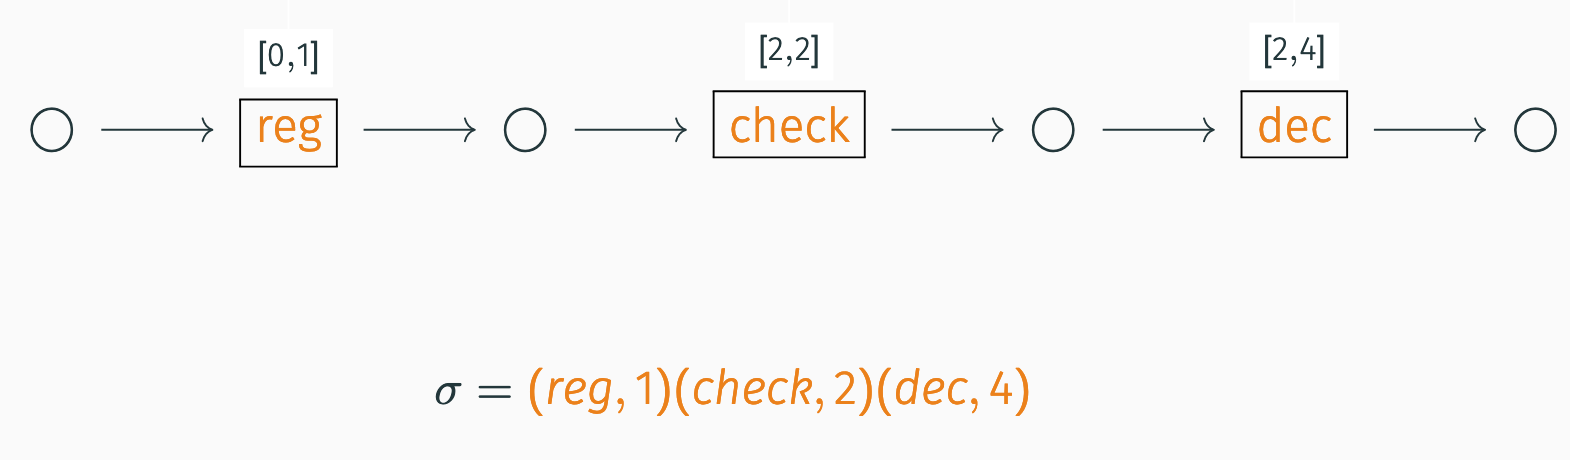
\includegraphics[width=5.5cm]{n3.png}
             \end{tabular}
    
    \end{tabular}
    $$cost(\gamma) = \sum_{i = 1}^{n}{|\gamma_i - \sigma_i|}$$
        \vfill 
%        
%         
%  change the parbox width as appropiate
             Consider the minimum cost of aligning an $i$-length prefix as a function of the value of the $i$-th timestamp, called $g_i$.

       $$g_i(d) = \min_{\tau|_i \in \mathcal{L}^i(N) \wedge \tau_i = d} cost(\tau|_i)$$ 
    \end{frame}
    
    \begin{frame}{Example}
\begin{tabular}{cl}  
         \begin{tabular}{c}
           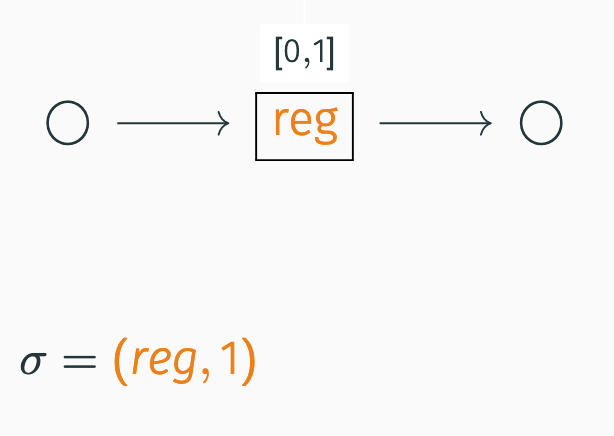
\includegraphics[width=4cm]{n1.png}
           \end{tabular}
           & \begin{tabular}{l}
             \parbox{0.4\linewidth}{%  change the parbox width as appropiate
  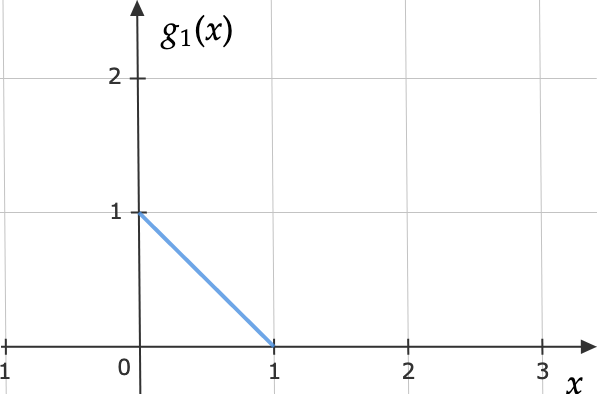
\includegraphics[width=5cm]{g1.png}
    }\end{tabular}
    
    \end{tabular}
             \vfill 
             $$g_1(d) = d_t(\alert{(reg,d) \to (reg,1)}) = |d - 1| = |d-\sigma_1|$$

    \end{frame}
    
    \begin{frame}{Stamp only algorithm for sequential models, continued}

 

        Split cost at the last letter to get the following recursion : 
        	%$$\min_{\tau|_{i+1} \in \mathcal{L}^{i+1}(N)}cost(\tau|_{i+1}) = \min_{\tau_{i+1} - \tau_i\in [a, b]} (|\tau_{i+1} - \sigma_{i+1}| + \min_{\tau|_i \in \mathcal{L}^i(N) }cost(\tau|_i))$$
        	$$g_{i+1}(d) = |d - \sigma_{i+1}| + \min_{d-d' \in [a,b]} g_i(d')$$
        	
        	 
        		
\begin{tabular}{cl}  
         \begin{tabular}{c}
        
           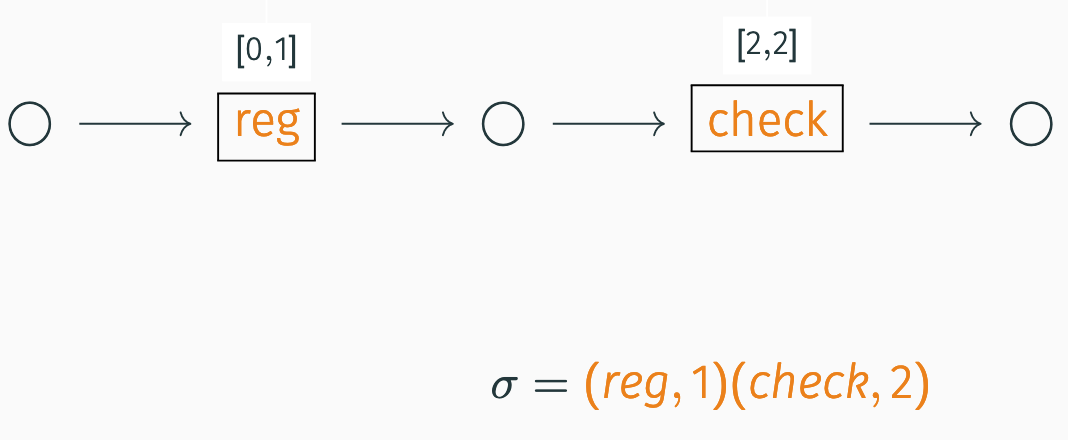
\includegraphics[width=5cm]{n2.png}
           
           \end{tabular}
           & \begin{tabular}{l}
             \parbox{0.4\linewidth}{%  change the parbox width as appropiate
  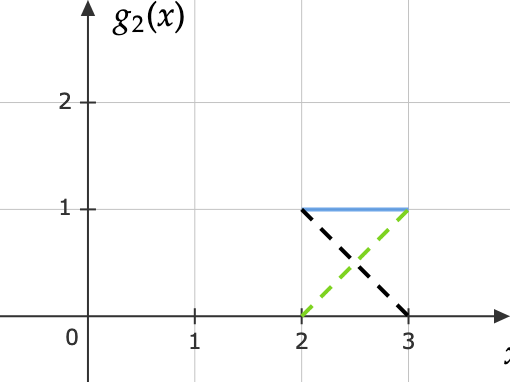
\includegraphics[width=5cm]{g2.png}
    }\end{tabular}
    
    \end{tabular}     
    
   $d_t(\alert{(reg,d-2)(check,d) \to (reg,1)(check,2)}) =$
   
   $g_2(d) = |d-2| + (g_1(d-2))$
    \vfill 
       The minimum cost of alignment $c = \min_{d} g_n(d)$.

    \end{frame}

%\begin{frame}[fragile]{Stamp only : Example}
%	Recall the process model $N$ : 
%		\\
%			\adjustbox{scale=0.6}{
%		\begin{tikzcd}
%	& {} && {} && {} && {\fbox{pay}} \\
%	\Huge\bigcirc & {\fbox{reg}} & \Huge\bigcirc & {\fbox{check}} & \Huge\bigcirc & {\fbox{dec}} & \Huge\bigcirc & {} & \Huge\bigcirc \\
%	&&&&&&& {\fbox{rej}}
%	\arrow["{[0, 1]}"{description, pos=0.2}, draw=white, from=2-2, to=1-2]
%	\arrow["{[0,1]}"{description, pos=0.1}, draw=white, from=1-8, to=2-8]
%	\arrow["{[0,0]}"{description, pos=0.1}, draw=white, from=3-8, to=2-8]
%	\arrow[from=2-1, to=2-2]
%	\arrow[from=2-2, to=2-3]
%	\arrow[from=2-3, to=2-4]
%%%%	\arrow[curve={height=-12pt}, from=2-7, to=1-8]
%	\arrow[curve={height=12pt}, from=2-7, to=3-8]
%	\arrow[curve={height=12pt}, from=3-8, to=2-9]
	%\arrow[curve={height=-12pt}, from=1-8, to=2-9]
	%\arrow["{[2,4]}"{description}, draw=white, from=2-6, to=1-6]
	%\arrow["{[2,2]}"{description, pos=0.2}, draw=white, from=2-4, to=1-4]
%\end{tikzcd}}

%\vfill 
%		The observed trace is $$\sigma = (reg, 1)\cdot (check, 2) \cdot (dec, 4) \cdot (pay, 6)$$
%		\vfill 
%        In the ith graph, the colour key is \textcolor{blue}{$g_i(d)$}, \textcolor{orange}{$\min_{d-d' \in [a,b]}$} $g_{i-1}(d')$, and \textcolor{green}{$|d - \sigma_i|$}
%\end{frame}

% \begin{frame}{ Diagrams: $g_1, g_2$}
%        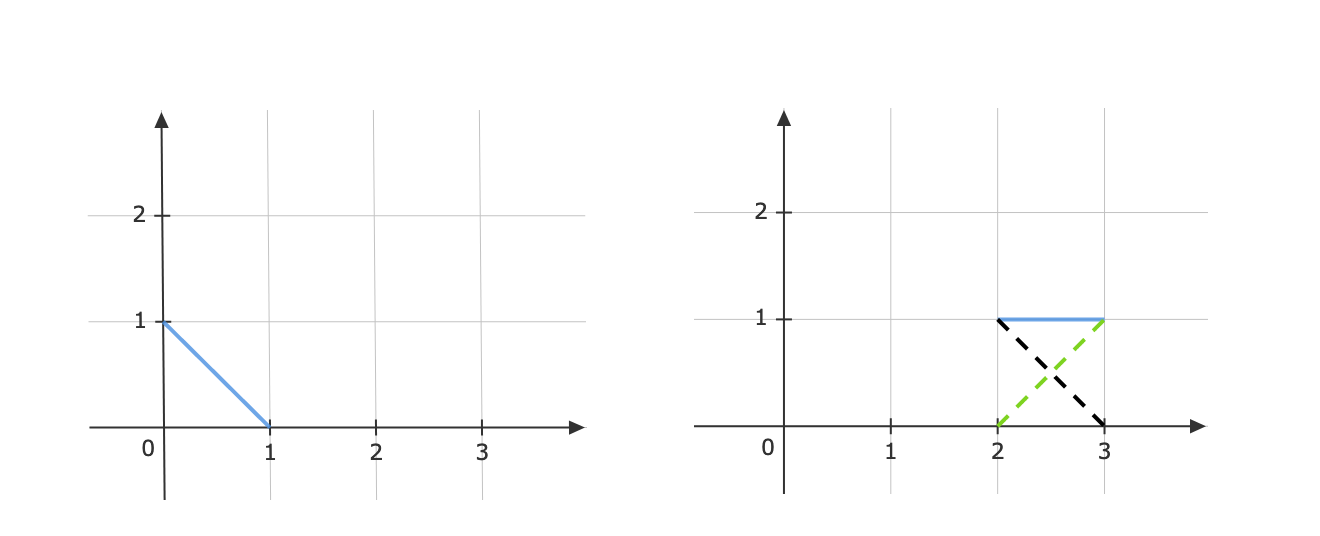
\includegraphics[width = \textwidth]{g12.png}
%\end{frame}

 \begin{frame}{Diagrams: $g_3, g_4$}
               In the ith graph, the colour key is \textcolor{blue}{$g_i(d)$}, \textcolor{orange}{$\min_{d-d' \in [a,b]}$} $g_{i-1}(d')$, and \textcolor{green}{$|d - \sigma_i|$}
               \vfill 
               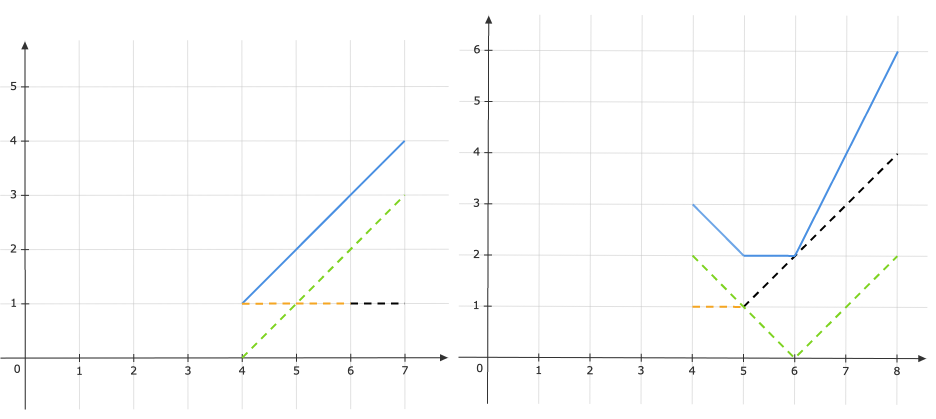
\includegraphics[width = \textwidth]{g34.png}

\end{frame}


%\begin{frame}{Mixed moves, $d_N$ : Computation}
%    \begin{itemize}
%        \item Firstly, we have a linear time algorithm for calculating the distance for sequential causal processes 
%        \vfill 
%        \item The algorithm is simple, but the proof of correctness was difficult
%    \end{itemize}
%\end{frame}

%\begin{frame}{Mixed moves, $d_N$ : Alignment}
%\metroset{block=fill}
%\begin{block}{Mixed Moves Alignment Result}
%    $\gamma_N = \gamma_\theta$
%\end{block}
%		\vfill 
%		 This gives us a linear algorithm for aligning under $d_N$, again, proving correctness was the hard part.  
%\end{frame}


\section{Conclusion}
\begin{frame}{Summary of Contributions}
\begin{itemize}
	\item We set the problem of General and Purely Timed Alignment for process models. 
	\vfill 
	\item We defined three metrics for timed words, and studied the purely timed alignment problem over them.  
	\vfill 
	\item For certain classes of process models, we provide original and efficient algorithms to solve purely timed alignment.

\end{itemize}
\end{frame}


\begin{frame}[fragile]{Future Directions : Back to GTAP}
	\begin{itemize}
		\item Approach 1 : First align letters, then timestamps
		\vfill 
		\item But consider : $(reg, 0)(check, 2)(dec, 4)\alert{(pay, 1004)}$
		
		\vfill
		
		\adjustbox{scale=0.6}{
		\begin{tikzcd}
	& {} && {} && {} && {\fbox{pay}} \\
	\Huge\bigcirc & {\fbox{reg}} & \Huge\bigcirc & {\fbox{check}} & \Huge\bigcirc & {\fbox{dec}} & \Huge\bigcirc & {} & \Huge\bigcirc \\
	&&&&&&& {\fbox{rej}}
	\arrow["{[0, 1]}"{description, pos=0.2}, draw=white, from=2-2, to=1-2]
	\arrow["{\alert{[0,1]}}"{description, pos=0.1}, draw=white, from=1-8, to=2-8]
	\arrow["{\alert{[1000,1000]}}"{description, pos=0.1}, draw=white, from=3-8, to=2-8]
	\arrow[from=2-1, to=2-2]
	\arrow[from=2-2, to=2-3]
	\arrow[from=2-3, to=2-4]
	\arrow[from=2-4, to=2-5]
	\arrow[from=2-5, to=2-6]
	\arrow[from=2-6, to=2-7]
	\arrow[curve={height=-12pt}, from=2-7, to=1-8]
	\arrow[curve={height=12pt}, from=2-7, to=3-8]
	\arrow[curve={height=12pt}, from=3-8, to=2-9]
	\arrow[curve={height=-12pt}, from=1-8, to=2-9]
	\arrow["{[2,4]}"{description}, draw=white, from=2-6, to=1-6]
	\arrow["{[2,2]}"{description, pos=0.2}, draw=white, from=2-4, to=1-4]
\end{tikzcd}}
		
	\vfill 
		\item Approach 1 is quite biased towards letters, but it is a start. 
	\end{itemize}
\end{frame}


\begin{frame}{Other Future Directions}
    \begin{itemize}
    	\item Conformance checking artefacts  should be adapted for time-aware systems.
	\vfill 
	\item Need algorithms that are both efficient and applicable to wider classes of models (branching models for $d_t$, computing and aligning under $d_N$)
	\vfill 
	\item Could further customise $d_N$
\end{itemize}
\end{frame}

\begin{frame}
    \Huge{\centerline{\textbf{Thank you!}}}
\end{frame}


%\appendix

\begin{frame}{Mixed Moves Alignment}
	
	Let us try to align the observed trace $(0, 3, 4)$ to the process trace $(0.5, 2.5, 3.5)$ under $d_N$

\vfill 
Intuitively,  we can assume a minimum cost run is left to right, or, \alert{chronological}. 
\vfill 
So our first move will have to incur a minimum cost of $0.5$ as we try to align $(0,3,4)$ to our process trace at the first position.
\vfill 
Ensuring a move is not counterproductive at a position is what we call \alert{co-operation}. 


\end{frame} 

\begin{frame}{Mixed Moves Alignment}

	Now we move on to move two, which will again incur a minimum cost of $0.5$. 
	\vfill 
	This unique choice of stamp that moves the local component as close as possible to the desired one indirectly represents what we define as \alert{stability}. 
	\vfill 
	Hence, the least cost alignment is $(0.5, 0, 1)(0, -0.5, 2)$, with total cost 1. 
	\vfill 
	In fact distance 1 is the best we can do here even in the mixed case. 
\end{frame} 
%----------------------------------------------------------------------------------------



\end{document}
